\documentclass[
	mode=present,
	paper=screen,
	orient=landscape,
	display=slides,
	style=simple
	]{powerdot}
\pdsetup{
logohook=t,
logopos={.06\slidewidth,.087\slideheight},
logocmd={
\includegraphics[height=.08\slideheight]{hi_logo.eps}} % 
}
\usepackage{epsfig}
\usepackage{amsbsy}
\usepackage{rotating}
\usepackage{graphicx}
\usepackage{natbib}
\usepackage{boxedminipage}
\usepackage{my_macros}
\usepackage{movie15}
\usepackage{rotate}
%\usepackage[monochrome]{color}
%\setlength{\unitlength}{1cm}
\renewcommand{\vec}[1]{{\mathbf #1}}

%%%%%%%%%%%%%%%%%%%%%%%%%%%%%%%%%%%%%%%%%%%%%%%%%%%%%%%%%%%%%%%%%%%%%%%%%%
%%% title
\title{Pilot, Rollout and Monte Carlo Tree Search Methods\\ for Combinatorial Optimization}
\author{{\bf Thomas Philip Runarsson}\\
{School of Engineering and Natural Sciences, University of Iceland} \\ 
\ \\
{\bf Marc Schoenauer ~~~ Mich\`ele Sebag}\\
{TAO, INRIA Saclay Île-de-France, 
Orsay, France} \\ {TAO, LRI, UMR CNRS 8623, Orsay, France} \\ {Microsoft Research-INRIA Joint Centre, Orsay, 
France}}
\date{20 January 2012}

%\email{novak@math.wisc.edu}
%\slideCaption{Kyle Novak}
%\Logo{
\includegraphics[height=.9cm]{hi_logo}}
\begin{document}

\maketitle

\section[slide=false]{Introduction}
%%%%%%%%%%%%%%%%%%%%%%%%%%%%%%%%%%%%%%%%%%%%%%%%%%%%%%%%%%%%%%%%%%%%%%%%%%
%%% slide
\begin{slide}[toc=,bm=]{Overview}
\tableofcontents[content=sections]
\end{slide}


%%%%%%%%%%%%%%%%%%%%%%%%%%%%%%%%%%%%%%%%%%%%%%%%%%%%%%%%%%%%%%%%%%%%%%%%%%
%%% slide
\begin{slide}{Sequential Decision Making Problems}


Many optimization problems may be formulated within a sequential decision making (dynamic programming) framework, this 
includes the shortest path, assignment, packing, scheduling, etc.\\
\ \\
\pause

A solution consist of $n$ components, or decisions selected one-at-a-time. For $n=1,\ldots,N$, the state of the $n$th 
stage is formed by the sequence of $n$ decisions: 
$$(u_1,u_2,\ldots,u_n)$$

\pause

For example, in \emph{job scheduling} decisions may involve selecting different dispatching heuristic or simply the 
job to be 
scheduled next.



\end{slide}

\section[slide=false]{Pilot and Rollout Algorithms}

%%%%%%%%%%%%%%%%%%%%%%%%%%%%%%%%%%%%%%%%%%%%%%%%%%%%%%%%%%%%%%%%%%%%%%%%%%
%%% slide
\begin{slide}{Rollout Algorithms (Bertsekas, Tsitsiklis, 1997)}

The key idea is to employ a given heuristic in the construction of an optimal cost-to-go
function approximation, which is then used in the spirit of the \emph{neuro-dynamic programming} and 
\emph{reinforcement learning} methodology.\\
\ \\
\pause

In particular, an optimal solution $(u_1^*,\ldots,u_N^*)$ can be obtained by
$$u_i^*=\arg\min_{u_i\in U_i(u_1^*,\ldots,u_{i-1}^*)}J^*(u_1^*,\ldots,u_{i-1}^*,u_i),\quad i=1,\ldots,N$$

\pause
The Rollout algorithm uses multiple \emph{heuristics} to provide an approximation of $J^*$ and so obtain a 
sub-optimal 
solution
$$\tilde{u}_i=\arg\min_{\tilde{u}_i\in 
U_i(\tilde{u}_1,\ldots,\tilde{u}_{i-1})}\tilde{J}(\tilde{u}_1,\ldots,\tilde{u}_{i-1},u_i),\quad i=1,\ldots,N$$


\end{slide}


\begin{slide}{Rollout Algorithms (Bertsekas, Tsitsiklis, 1997)}

The name “rollout policy” was used by Tesauro (Tesauro and Galperin, 1996) in connection with one of his
simulation-based computer backgammon algorithms, also known as \emph{trajectory sampling} (Sutton and Barto, 1998)\\
\ \\
\pause


There are different versions of the Rollout algorithm, one in particular looks at all downstream neighbour states, 
$\mathcal{N}(u_{i-1})$, of the partial solution $(\tilde{u}_1,\ldots,\tilde{u}_{i-1})$: and uses a default heuristic 
to 
generate 
a complete solution with cost $C(j)$. \\
\ \\
\pause

The decision made is then
 
$$\tilde{u}_i=\arg\min_{j\in 
\mathcal{N}(\tilde{u}_{i-1})}C(j)$$


\end{slide}


\begin{slide}{Pilot Method (Duin and Vo\ss, 1994.)}

\underline{P}referred \underline{I}terative \underline{LO}ok ahead \underline{T}echnique.

\begin{itemize}
\item The idea is to add one-step look-ahead and so apply greedy heuristics from different starting points. \\  \ \\
\pause
\item The procedure is applied repeatedly, effectively building a tree. \\ \ \\ \pause
\item This procedure is not unlike strategies used in game playing programs, that search a game trees for good 
moves.\\ \ \\ \pause
\item Essentially equivalient to the Rollout algorithm, but motivated differently.
\end{itemize}

\end{slide}



\section[slide=false]{Monte Carlo Methods}
%%%%%%%%%%%%%%%%%%%%%%%%%%%%%%%%%%%%%%%%%%%%%%%%%%%%%%%%%%%%%%%%%%%%%%%%%%
%%% slide\
\begin{slide}{Monte Carlo Rollouts}

\begin{itemize}
\item The idea here is to complete solutions randomly from partial solutions $(u_1,\ldots,u_{i-1})$.\\ \ \\ \pause
\item This is more efficient than using problem specific heuristics, but also less effective.\\ \ \\ \pause
\item Heuristic rollouts are sequentially consistent, random solutions are not. This requires us to store the 
best sequence found globally during a run.
\end{itemize}


\end{slide}

\begin{slide}{Monte-Carlo Tree Search}
\begin{minipage}[c]{1.25in}
	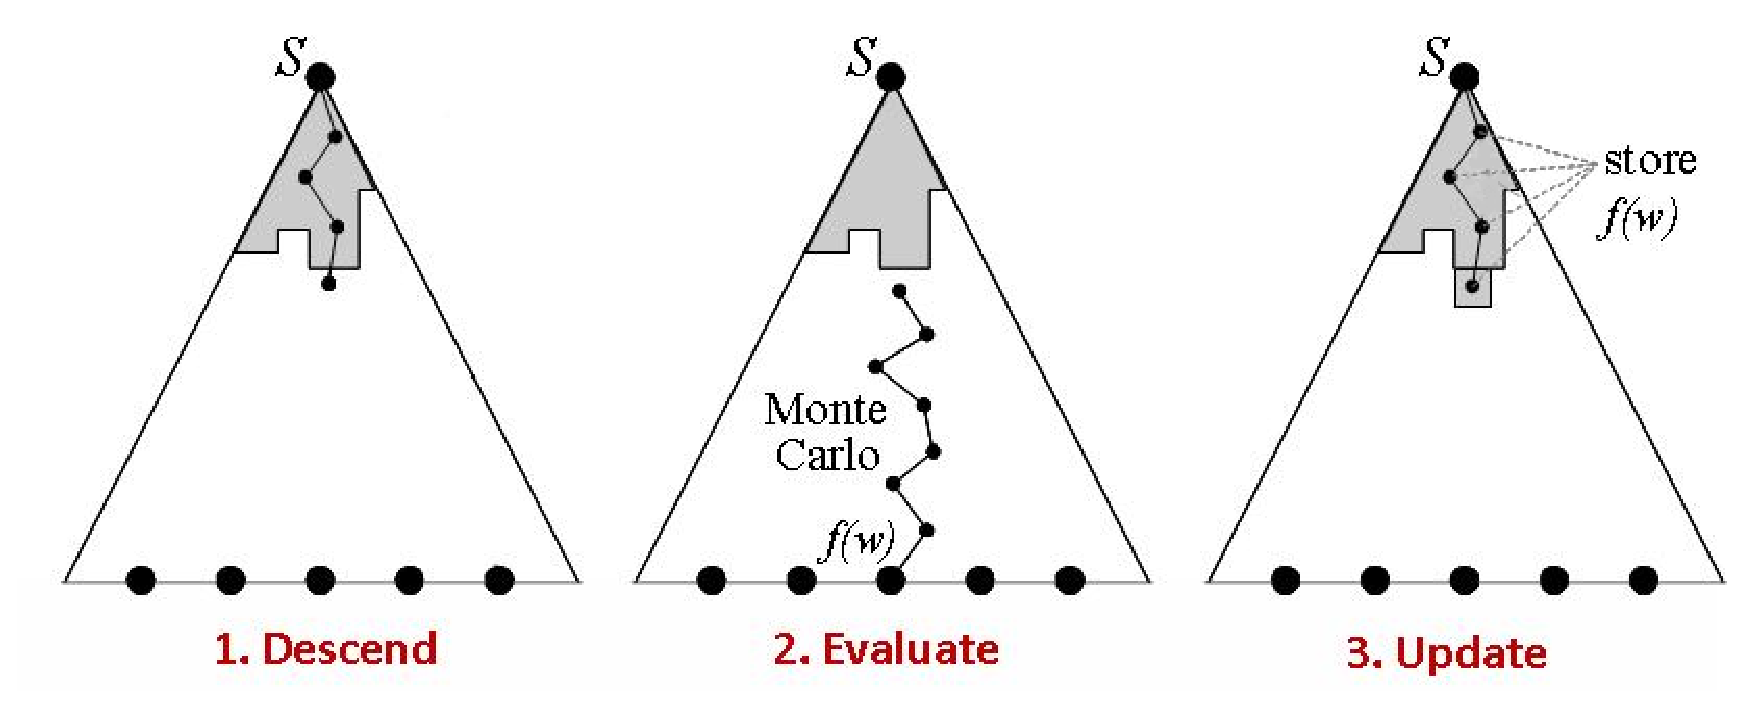
\includegraphics[width=10cm]{mcts.eps}
\end{minipage}
\begin{itemize}
\item A tree is asymmetrically grown toward the most promising region (grey part explored at a previous 
iterations).\pause
\item Tree descended using an exploration/exploitation policy until an unexplored leaf found.\pause
\item Node added to the tree and solution completed randomly.\pause
\item Solution back-propagated to nodes on the path taken.
\end{itemize}
\end{slide}

\begin{slide}{Monte-Carlo Tree Search}
The sought solution is the one with best payoff (as opposed to the one with best
payoff on average); the decision problem is therefore a \emph{$\max~k$-armed bandit problem}.\\
\ \\
\pause

There exist at least two different approaches to tackling this problem (Streeter 2006, Rimmel 2009), but require 
additional parametric tuning, so here we simply use an $\epsilon$-greedy trial allocation policy when traversing down 
the tree.\\ \ \\
\pause
The Pilot and Rollout algorithms can be considered a special case of the Monte Carlo Tree Search (MCTS). \\ \ \\

\pause
The Dyna$-2$ (Silver, Sutton and M\"uller, 2008) architecture subsumes a large family of learning and search 
algorithms, including MCTS.


\end{slide}


\section[slide=false]{Experimental Study}
\begin{slide}{Job Shop Scheduling Heuristics}

Instance generator using a uniform random generator for processing times $U(1,200)$ (integer values only).\\
\ \\

\pause

Size of jobs $6\times 6$, $10\times 10$ and $14\times 14$ can be solved using a specialized branch \& bound procedure 
any size greater than this cannot be solved in any reasonable time. \pause 
One hundred independent instance were created and the algorithm run once per instance.\pause \ Number of rollouts 
varied.\\
\ \\
\pause



Best single dispatching heuristics are:\\ (in order of performance)
\begin{itemize}
\item Most works remaining (MWKR), 
\item Least Operation Number (LOPN)
\item Shortest processing time (SPT)
\end{itemize}



\end{slide}


\begin{slide}{Pilot Algorithm}

The original heuristics improved upon using the Pilot algorithm, the tables show the ratio of objective value 
(Makespan for the scheduling problem) against the known optimal solution.
{\footnotesize
 \begin{center}
\begin{tabular}{l|l|ccccc|c}
Instance & Heuristic & min & mean & median & stdev & max & \#opt\\\hline
$ 6\times  6$ & MWKR & 1.000 & 1.155 & 1.151 & 0.084 & 1.384 & 2 \\
& Pilot(MWKR) & 1.000 & 1.025 & 1.014 & 0.029 & 1.104 & 33 \\\hline
& SPT & 1.137 & 1.399 & 1.390 & 0.150 & 1.816 & 0 \\
& Pilot(SPT) & 1.000 & 1.052 & 1.049 & 0.045 & 1.265 & 14\\\hline
$10\times 10$ & MWKR & 1.096 & 1.228 & 1.222 & 0.069 & 1.430 & 0 \\
& Pilot(MWKR) & 1.004 & 1.082 & 1.083 & 0.035 & 1.158 & 0\\\hline
& SPT & 1.303 & 1.654 & 1.644 & 0.166 & 2.161 & 0 \\
& Pilot(SPT) & 1.063 & 1.172 & 1.168 & 0.048 & 1.296 & 0\\\hline
$14\times 14$ & MWKR & 1.159 & 1.264 & 1.261 & 0.052 & 1.399 & 0 \\
& Pilot(MWKR) & 1.046 & 1.129 & 1.129 & 0.034 & 1.230 & 0\\\hline
& SPT & 1.584 & 2.012 & 2.015 & 0.244 & 2.721 & 0 \\
& Pilot(SPT) & 1.153 & 1.286 & 1.283 & 0.060 & 1.517 & 0\\\hline
\end{tabular}
 \end{center}}



\end{slide}


\begin{slide}{Monte Carlo Tree Search}

The performance of the MCTS is superior for problem sizes less than $14 \times 14$, at this point the Pilot method 
will give a better result, when using the MWRM and LOPN heuristics.

{\footnotesize
 \begin{center}
\begin{tabular}{l|l|ccccc|c}
Instance & Heuristic & min & mean & median & stdev & max & \#opt\\\hline
$ 6\times  6$ & MWKR & 1.000 & 1.155 & 1.151 & 0.084 & 1.384 & 2 \\
& Pilot(MWKR) & 1.000 & 1.025 & 1.014 & 0.029 & 1.104 & 33 \\
& MCTS & 1.000 & 1.007 & 1.000 & 0.017 & 1.082 & 72\\\hline
$10\times 10$ & MWKR & 1.096 & 1.228 & 1.222 & 0.069 & 1.430 & 0 \\
& Pilot(MWKR) & 1.004 & 1.082 & 1.083 & 0.035 & 1.158 & 0\\
& MCTS & 1.000 & 1.070 & 1.070 & 0.032 & 1.135 & 2\\\hline
$14\times 14$ & MWKR & 1.159 & 1.264 & 1.261 & 0.052 & 1.399 & 0 \\
& Pilot(MWKR) & 1.046 & 1.129 & 1.129 & 0.034 & 1.230 & 0\\
& MCTS & 1.064 & 1.232 & 1.223 & 0.065 & 1.471 & 0 \\\hline \pause
& Pilot(LOPN) & 1.078 & 1.145 & 1.142 & 0.033 & 1.248 & 0 \\
& Pilot(SPT) & 1.153 & 1.286 & 1.283 & 0.060 & 1.517 & 0\\\hline
\end{tabular}
 \end{center}}


\end{slide}



\section[slide=false]{Summary and Future Work}

\begin{slide}{Discussion}

\begin{itemize}
 \item MC rollouts are considerably faster than using Heuristic rollouts, so we could have more of them.\pause
 \item For larger problems the MC rollouts need to be biased towards more favourable regions in the search space.\pause
 \item The current best found global solution may suggest an alternative decision at some decision stages.\pause
\end{itemize}

Some work in progress

\begin{itemize}
\item Use a $\max$-bandit trial allocations strategy when descending the tree.\pause
\item Implementing the rave, that is learn an approximate $J^*$ on-line, can be used to complement the 
exploration- exploitation phase,\pause and/or use it to bias the MC rollouts.\pause
\item Progressive widening was not used here, but would be required for other application (branching factor low here).
\end{itemize}



\end{slide}


\begin{slide}{Thank you}
\vspace{1in}
\begin{center}
Questions?
\end{center}
\end{slide}


\end{document}

\section[slide=false]{Semi-classical Limit}
%%%%%%%%%%%%%%%%%%%%%%%%%%%%%%%%%%%%%%%%%%%%%%%%%%%%%%%%%%%%%%%%%%%%%%%%%%
%%% slide
\begin{slide}{Wigner Equation}
Schr\"odinger equation
\[
	\mathcal{S} \Psi(x,t) = \D{}{t} \Psi(x,t) + \frac{\eps}{2i} \Delta \Psi(x,t) - \frac{1}{\eps i} V(x) \Psi(x,t) = 0
\]

Wigner distribution function
\[
	f(x,p,t) = \mathcal{W}[\Psi,\Psi] = \intI \conj \Psi(x-\tfrac12\eps y,t)\Psi(x+\tfrac12\eps y,t)e^{ipy}\,dy
\]

Wigner equation: 
$\mathcal W[\mathcal S \Psi,\Psi] + \mathcal W[\Psi,\mathcal S \Psi] = 0$
\pause
\[
	\D{}{t} f + p\grad f + \Theta = 0	\WHERE
\]
\[
	\Theta = -\frac{1}{\eps i} \int \left[ V(x+\tfrac12\eps y) - V(x - \tfrac12 \eps y) \right]  \hat f(x,y,t)   e^{-ipy} \,dy
\]
\end{slide}

%%%%%%%%%%%%%%%%%%%%%%%%%%%%%%%%%%%%%%%%%%%%%%%%%%%%%%%%%%%%%%%%%%%%%%%%%%
%%% slide
\begin{slide}{Semiclassical limit}
\[
	\Theta = \grad_xV \cdot \grad_p f - \frac{1}{\eps i} \sum_{n=1}^\infty  \frac{(-1)^n \(\frac{\eps}{2}\)^{2n}}{(2n+1)!} \grad_x^{2n+1} V \grad^{2n+1}_p f		
\]
\pause
For	$V(x)$ smooth, when $\eps \to 0$ 
\[	
	\Theta \to  \grad_xV \cdot \grad_p f(x,p,t)
\]

Liouville equation:
\ceqnbox{pdlblue}{\dd{}{t}f  = \D{}{t}f  + \frac{p}{m} \grad_x f  - \grad_xV \cdot \grad_p f  = 0} 

\pause
Characteristics $\equiv$ Hamiltonian system: 
\begin{align*}
	\dot{\mathbf{x}} &= \frac{\mathbf{p}}{m}	\\
	\dot{\mathbf{p}} &= -\grad_x V(x) = \mathbf{F}
\end{align*}
\end{slide}

%%%%%%%%%%%%%%%%%%%%%%%%%%%%%%%%%%%%%%%%%%%%%%%%%%%%%%%%%%%%%%%%%%%%%%%%%%
%%% slide
%\begin{slide}{Schr\"odinger/Liouville}
%\begin{align*}
%	\( \D{}{t} + \frac{\eps}{2mi}\Delta - \frac{1}{\eps i} V(x)\) \Psi(x,t) &= 0\\
%	\(\D{}{t} + \frac{p}{m} \grad_x  - \grad_x V \cdot \grad_p\) f(x,p,t)  &= 0 
%\end{align*}
%	wave 	 	particle\\
%	linear in $\Psi$  linear in $f$
%	$p,x$ dependent   independent\\	
%\begin{align*}
%	|\Psi(x,t)|^2 &= \intI f(x,p,t) \,dp\\
%	|\hat \Psi(x,t)|^2 &= \intI f(x,p,t) \,dx
%\end{align*}
%\end{slide}

%%%%%%%%%%%%%%%%%%%%%%%%%%%%%%%%%%%%%%%%%%%%%%%%%%%%%%%%%%%%%%%%%%%%%%%%%%
%%% slide
\begin{slide}{Why not use the Schr\"odinger Equation?}
Liouville equation
\begin{itemize}
		\item Arbitrary particle distribution, \emph{but}
		\item No wave phenomena:	tunneling, resonance, partial transmission/reflection, interference
	\end{itemize}
\pause
Schr\"odinger equation
\begin{itemize}
	\item Accurately models particle at any scale, \emph{but}
	\item	Single particle ($x$ and $p$ distribution are not independent)
	\item	Numerically, we must resolve the de~Broglie wavelength. 
		Typically, $\Delta x = O(\eps/p)$ or $\Delta x = o(\eps/p)$  
	\item	Numerically, difficult to implement boundary conditions
\end{itemize}
	
\pause

\vspace{12pt}
\fcolorbox{pdlblue}{white}{
\begin{minipage}{.5in}
\emph{Idea!}
\end{minipage}
\begin{minipage}{2.5in}
Use Liouville equation globally. \\
Use Schr\"odinger equation locally.
\end{minipage}
}

\end{slide}


\section[slide=false]{Mixed Model}{
%%%%%%%%%%%%%%%%%%%%%%%%%%%%%%%%%%%%%%%%%%%%%%%%%%%%%%%%%%%%%%%%%%%%%%%%%%
%%% slide
\begin{slide}{How do we do it?}
Coupling a quantum barrier with a Liouville
\begin{itemize}
	\item Solve the time-independent Schr\"odinger equation for the a local barrier/well
	\item	Use the solution to determine scattering information
	\item Solve the Liouville equation everywhere else
	\item Use scattering information to connect across the barrier 
\end{itemize}
	
	Previous research
	\begin{itemize}
		\item N. Ben Abdallah, P. Degond and I.M. Gamba (2002)
		\item S. Jin and X. Wen (2005)
	\end{itemize}

Simplifying assumptions
\begin{itemize}
	\item We work in 1-d
	\item Particle moves instantaneously across the barrier
	\item Barrier is sufficiently local
	\item Particle has no phase information (no long range interaction)
\end{itemize}
\end{slide}
%%%%%%%%%%%%%%%%%%%%%%%%%%%%%%%%%%%%%%%%%%%%%%%%%%%%%%%%%%%%%%%%%%%%%%%%%%
%%% slide
%\begin{slide}{Outline}
%\begin{itemize}
%	\item[] Solve the Schr\"odinger equation\\[12pt]
%	\item[]	Determine scattering information\\[12pt]
%	\item[] Solve the Liouville equation\\[12pt]
%	\item[] Connect across the barrier\\[12pt]
%\end{itemize}
%\end{slide}


\section[slide=false]{Schr\"odinger Solution}
%%%%%%%%%%%%%%%%%%%%%%%%%%%%%%%%%%%%%%%%%%%%%%%%%%%%%%%%%%%%%%%%%%%%%%%%%%
%%% slide
\begin{slide}{Transfer Matrix}
\onslide*{1}{
Solve $\frac{\eps^2}{2m} \Delta \Psi  - V(x) \Psi = E \Psi$ where
\[
	V(x) = \begin{cases}
		V_1, & x\in\mathcal{C}_1\\
		V_\mathcal{Q}(x), & x\in\mathcal{Q}\\
		V_2, & x\in\mathcal{C}_2
		\end{cases}	
	\]
	\begin{center}
		\psfrag{A}{}
		\psfrag{B}{}
		\psfrag{V1}{$\mathcal{C}_1$}
		\psfrag{V2}{$\mathcal{C}_2$}
		\psfrag{VQ}{$\mathcal{Q}$}
%		\includegraphics[width=3in]{single_barrier}
\end{center}
}
\onslide*{2-3}{
\begin{flushleft}
$	
	\text{In } \mathcal{C}: \Psi(x) = \begin{cases}
		a_{1} e^{i\kappa_{1} x} + b_{1} e^{-i\kappa_{1} x}, & x\in\mathcal{C}_1\\
		b_{2} e^{i\kappa_{2} x} + b_{2} e^{-i\kappa_{2} x}, & x\in\mathcal{C}_2
		\end{cases}
$		
\begin{flushright}
$\WHERE \kappa_j = \sqrt{p^2 - 2mV_j}/\eps$
\end{flushright}
	\end{flushleft}
	\begin{center}
		\psfrag{A}[c]{$\omat{a_1 \rightarrow\\ b_1\leftarrow}$}
		\psfrag{B}[c]{$\omat{ \rightarrow a_2 \\\leftarrow  b_2}$}
		\psfrag{V1}{$\mathcal{C}_1$}
		\psfrag{V2}{$\mathcal{C}_2$}
		\psfrag{VQ}{$\mathcal{Q}$}
%		\includegraphics[width=3in]{single_barrier}
		\end{center}
}
\onslide*{3}{
		In $\mathcal{Q}$:  linear, 2nd-order BVP, so $\pmat{a_2\\b_2} = \mathsf{M} \pmat{a_1 \\ b_1}$		
}
\onslide*{4-5}{
	Multiple barriers\\[12pt]
	\begin{center}
		\psfrag{A}[c]{\small$\omat{a_1 \rightarrow\\ b_1\leftarrow}$}
		\psfrag{B}[c]{\small$\omat{ \rightarrow a_n \\\leftarrow  b_n}$}
		\psfrag{M1}{$\mathsf{M}_1$}
		\psfrag{M2}{$\mathsf{M}_2$}
		\psfrag{...}{$\dots$}
		\psfrag{MN}{$\mathsf{M}_n$}
		\includegraphics[width=3in]{multiple_barriers}	
		$\pmat{a_n\\b_n} = \underbrace{\mathsf{M_n} \mathsf{M}_{n-1} \cdots \mathsf{M_1}}_{\displaystyle \mathsf{M}}\pmat{a_1 \\ b_1}$
	\end{center}
}
\onslide*{5}{
		\vspace{12pt}
		Two simple barriers
		\begin{itemize}
			\item Step ($\mathsf{D}$)
			\item Translation ($\mathsf{P}$)
		\end{itemize}
		}
\onslide*{6}{
	Arbitrary barrier
	\begin{center}
	\includegraphics[width=3in]{steps}
	\end{center}
	\begin{align*}
		\mathsf{M}_j &= \mathsf{P}^{1/2}_{j+1}\mathsf{D}_j\mathsf{P}^{1/2}_j\\
		\mathsf{D}_j &= \tfrac12\pmat{1+\kappa_{j-1}/\kappa_j & 1-\kappa_{j-1}/\kappa_j  \\ 1-\kappa_{j-1}/\kappa_j  & 1+\kappa_{j-1}/\kappa_j }\\
		\mathsf{P}_j &= \pmat{\exp(i\Delta x \kappa_j) & 0 \\ 0 & \exp(-i\Delta x \kappa_j)}
	\end{align*}
}
\end{slide}


%%%%%%%%%%%%%%%%%%%%%%%%%%%%%%%%%%%%%%%%%%%%%%%%%%%%%%%%%%%%%%%%%%%%%%%%%%
%%% slide
\begin{slide}{Scattering Matrix}
\begin{center}
		\psfrag{A}[c]{$\omat{a_1 \rightarrow\\ b_1\leftarrow}$}
		\psfrag{B}[c]{$\omat{ \rightarrow a_2 \\\leftarrow  b_2}$}
		\psfrag{V1}{}
		\psfrag{V2}{}
		\psfrag{VQ}{}
		\includegraphics[width=3in]{single_barrier}
	\end{center}
\[
\begin{array}{cc}
\text{Transfer matrix}&\qquad\text{Scattering matrix}\\	
\pmat{a_2\\b_2} = \mathsf{M} \pmat{a_1 \\ b_1}&\qquad	\pmat{b_1\\a_2} = \mathsf{S} \pmat{a_1 \\ b_2}\\
\end{array}
\]
	
\begin{align*}
	\mathsf{M}  &=  \pmat{m_{11} & m_{12} \\ m_{21} & m_{22}}\\
	\mathsf{S} &= \pmat{r_1 & t_2 \\ t_1 & r_2}  = \pmat{-m_{21}/m_{22} & 1/m_{22} \\ \det\mathsf{M}/m_{22} & m_{12}/m_{22}}
\end{align*}
\end{slide}

%%%%%%%%%%%%%%%%%%%%%%%%%%%%%%%%%%%%%%%%%%%%%%%%%%%%%%%%%%%%%%%%%%%%%%%%%%
%%% slide
\begin{slide}{Current Density}
Schr\"odinger equation
\[
	\mathcal{S} \Psi(x,t) = \D{}{t} \Psi(x,t) + \frac{\eps}{2i} \eps \Delta \Psi(x,t) -\frac{1}{\eps i} V(x) \Psi(x,t) = 0
\]
Consider:
\[
	2 \Re[\conj \Psi \mathcal{S} \Psi ] = \conj \Psi \mathcal{S} \Psi  + \Psi \conj{\mathcal{S} \Psi} =0
\]
\pause
Continuity equation
\[
	\D{}{t}\rho(x,t) + \nabla \cdot J = 0
\]
where probability current density $J = \eps \Im[\conj \Psi \grad \Psi]$
\end{slide}


%%%%%%%%%%%%%%%%%%%%%%%%%%%%%%%%%%%%%%%%%%%%%%%%%%%%%%%%%%%%%%%%%%%%%%%%%%
%%% slide
\begin{slide}{Scattering Coefficients}
\begin{minipage}{2.5in}
$\Psi = \begin{cases}
	a_{1} e^{i\kappa_{1} x} + b_{1} e^{-i\kappa_{1} x}, & x\in\mathcal{C}_1\\ 
	a_{2} e^{i\kappa_{2} x} + b_{2} e^{-i\kappa_{2} x}, & x\in\mathcal{C}_1
	\end{cases}$ 
\end{minipage}
\begin{minipage}{1.4in}
\begin{center}
		\psfrag{A}[c]{$\begin{smallmatrix} a_1 \rightarrow \\ b_1 \leftarrow \end{smallmatrix}$}
		\psfrag{B}[c]{$\begin{smallmatrix} \rightarrow a_2 \\ \leftarrow b_2 \end{smallmatrix}$}
		\psfrag{V1}{}
		\psfrag{V2}{}
		\psfrag{VQ}{}
		\includegraphics[width=1.4in]{single_barrier}
	\end{center}
\end{minipage}

So,
\[
	J(x) = \eps \Im[\conj \Psi \grad \Psi] = 
	\begin{cases}
	\kappa_1 (|a_1|^2 - |b_1|^2),& x\in\mathcal{C}_1\\
	\kappa_2 (|a_2|^2 - |b_2|^2),& x\in\mathcal{C}_2
	\end{cases}	
\]
\pause
Particle incident from left: $b_2 = 0$ then $a_2 = t_1a_1$ and $b_1 = r_1a_1$
\[
	J(x) = \begin{cases}
	\kappa_1 |a_1|^2(1 - |r_1|^2), x\in\mathcal{C}_1\\
	\kappa_2 |a_2|^2 |t_1|^2, x\in\mathcal{C}_2
	\end{cases}	
\]
\pause
\fcolorbox{pdlblue}{white}{
\begin{minipage}{3in}
\begin{tabular}{ll}
Reflection probability & $R_1 = |r_1|^2$\\
Transmission probability & $T_1 = (\kappa_2/\kappa_1) |t_1|^2$
\end{tabular}
\end{minipage}
}
\end{slide}

%%%%%%%%%%%%%%%%%%%%%%%%%%%%%%%%%%%%%%%%%%%%%%%%%%%%%%%%%%%%%%%%%%%%%%%%%%
%%% slide
\begin{slide}{Resonance and Tunneling}
\psfrag{Transmission}{\tiny Transmission}
\psfrag{Momentum}{\tiny Momentum}
\onslide*{1-3}{Rectangular potential with height = $1/2$ and width $2\eps$\\[12pt]}
\onslide*{4-6}{Rectangular potential with height = $-1/2$ and width $8\eps$\\[12pt]}
\onslide*{1}{Step up}
\onslide*{2}{Step up + step down \textbf{independently}}
\onslide*{3}{Step up + step down \textbf{combined}}
\onslide*{4}{Step down}
\onslide*{5}{Step down + step up \textbf{independently}}
\onslide*{6}{Step down + step up \textbf{combined}}
\begin{center}
\onslide*{1}{\includegraphics[width=3in,height=2in]{pic1}}
\onslide*{2}{\includegraphics[width=3in,height=2in]{pic2}}
\onslide*{3}{\includegraphics[width=3in,height=2in]{pic3}}
\onslide*{4}{\includegraphics[width=3in,height=2in]{pic4}}
\onslide*{5}{\includegraphics[width=3in,height=2in]{pic5}}
\onslide*{6}{\includegraphics[width=3in,height=2in]{pic6}}
\end{center}
\end{slide}


\section[slide=false]{Liouville Solution}

%%%%%%%%%%%%%%%%%%%%%%%%%%%%%%%%%%%%%%%%%%%%%%%%%%%%%%%%%%%%%%%%%%%%%%%%%%
%%% slide
\begin{slide}{Semi-classical Liouville Equation}
\begin{minipage}{1.25in}
\begin{center}
\includegraphics[width=1in]{reflect_transmit}
\end{center}
\end{minipage}
\begin{minipage}{2.5in}
Bicharacteristics:
\begin{itemize}
	\item Classical particle is either transmitted \textbf{or} reflected
	\item Quantum particle is generally both transmitted \textbf{and} reflected
\end{itemize}
\end{minipage}
\begin{itemize}
	\item	Hamiltonian $p^2/2m - V(x)$ constant along characteristics
	\item	Particle density	$f(x,p,t)$ carried along bicharacteristics
	\end{itemize}
\end{slide}


%%%%%%%%%%%%%%%%%%%%%%%%%%%%%%%%%%%%%%%%%%%%%%%%%%%%%%%%%%%%%%%%%%%%%%%%%%
%%% slide
\begin{slide}{Finite Difference Scheme}
\onslide*{1}{
\ceqnbox{pdlblue}{f_t + v f_x - V_x f_v = 0}
Grid points at $(x_i,v_j)$.
Barrier at $x_{Z+1/2}$.
\[
	 \partial_t f_{ij} + v_j \cdot \partial_x f_{ij} - \partial_x V_i \cdot \partial_v f_{ij} = 0
\]
where 
$
	\partial_x f_{ij} = (f_{i+1/2,j} - f_{i-1/2,j})/\Delta x
$

\psfrag{x_0}{\scriptsize$x_{i-1}$}
\psfrag{x_1}{\scriptsize$x_{i}$}
\psfrag{x_2}{\scriptsize$x_{i+1}$}
\psfrag{f_0-}[l][r]{\scriptsize$f_{i-1/2}$}
\psfrag{f_0+}[c]{}
\psfrag{f_1-}[l][r]{\scriptsize$f_{i+1/2}$}
\psfrag{f_1+}[c]{}
\begin{center}
\includegraphics[width = 3in]{upwind}
\end{center}

Stability requires upwinding to approximate $f_{i\pm1/2}$\\
}

\onslide*{2}{
\psfrag{x_0}{\scriptsize$x_{i-1}$}
\psfrag{x_1}{\scriptsize$x_{i}$}
\psfrag{x_2}{\scriptsize$x_{i+1}$}
\psfrag{f_0-}{\scriptsize$f^-_{i-1/2}$}
\psfrag{f_0+}{\scriptsize$f^+_{i-1/2}$}
\psfrag{f_1-}{\scriptsize$f^-_{i+1/2}$}
\psfrag{f_1+}{\scriptsize$f^+_{i+1/2}$}
\begin{center}
\includegraphics[width = 3in]{upwind}
\end{center}

Where $f_{i\pm1/2}$ is continuous, $f_{i\pm1/2}^{-} = f_{i\pm1/2}^{+}$
\begin{align*}
	\partial_x f_{ij} &= \frac{f^{-}_{i+1/2,j} - f^{-}_{i-1/2,j}}{\Delta x}	\quad\text{if}\quad v_j>0\\
	\partial_x f_{ij} &= \frac{f^{+}_{i+1/2,j} - f^{+}_{i-1/2,j}}{\Delta x}	\quad\text{if}\quad v_j<0
\end{align*}
}
\end{slide}

\begin{slide}{Barrier Interface}
At the quantum barrier $x_{Z+1/2}$, we need to incorporate information from two bicharacteristics.\\[12pt]
	
Barrier interface condition
\begin{align*}
	f^+_{Z+1/2,j} &= R_{-j}f^+_{Z+1/2,-j}  +  T_{-j}f^-_{Z+1/2,w(j)}   \\
	f^-_{Z+1/2,j} &= R_{-j}f^-_{Z+1/2,-j}  +  T_{-j}f^+_{Z+1/2,w(j)}.
\end{align*}
 
\onslide*{1}{
\begin{center}
\psfrag{rj}[r][r]{\scriptsize$j$}
\psfrag{r-j}[r][r]{\scriptsize$-j$}
\psfrag{rR-j}[r][r]{\scriptsize$R_{-j}$}
\psfrag{rT-j}[r][r]{\scriptsize$T_{-j}$}
\psfrag{r-w-j}[r][r]{\scriptsize$w_{j}$}
\psfrag{lj}[l]{\scriptsize$j$}
\psfrag{l-j}[l]{\scriptsize$-j$}
\psfrag{lR-j}[l]{\scriptsize$R_{-j}$}
\psfrag{lT-j}[l]{\scriptsize$T_{-j}$}
\psfrag{l-w-j}[l]{\scriptsize$w_{j}$}
\includegraphics[width = 3in]{barrier_interface}
\end{center}
}

\onslide*{2}{
We use the approximation
\[
	T_{-j}f^+_{Z+1/2,w(j)} = \frac{1}{v_j \Delta v}  \int_{w(v_{j-1/2})}^{w(v_{j+1/2})} T(v) v f^- \,dv 
\]
where we use Hamiltonian to determine $w$
\[
	w(v_{\pm|j|)} =  \pm \sqrt{v_j^2 \pm 2(V_{Z+1/2}^+ - V_{Z+1/2}^-)}
\]
}
\end{slide}

%%%%%%%%%%%%%%%%%%%%%%%%%%%%%%%%%%%%%%%%%%%%%%%%%%%%%%%%%%%%%%%%%%%%%%%%%%
%%% slide
\begin{slide}{2nd order method}
Piecewise linear:
\begin{align*}
	f_{i-1/2,j}^{+}  &= f_{i,j} - \tfrac12 \(1- \lambda_j\) \Delta x \sigma^x_{ij}	\\
	f_{i+1/2,j}^{-}  &= f_{i,j} + \tfrac12 \(1- \lambda_j\) \Delta x  \sigma^x_{ij}
\end{align*} with the slope $\sigma^x_{ij}$ calculated using the Van~Leer slope limiter 
\[
	\sigma^x_{ij} = \( \frac{f_{ij} - f_{i-1,j}}{\Delta x}\) 
	\phi \(  \frac{ f_{i+1,j} - f_{ij} }{f_{ij} - f_{i-1,j} } \) 
\WHERE
	\phi(\theta) = \frac{\theta + |\theta|}{1+|\theta|}
\]
and the Courant number $\lambda_j = |v_j| \Delta t / \Delta x$\\[12pt]

\begin{flushleft}
\fcolorbox{pdlblue}{white}{
%\begin{minipage}{4in}
%Since this calculation uses values on both sides of the barrier, the slope needs to be modified at the %barrier\emph{!}
%\end{minipage}
We can't do this directly across at the barrier\emph{!}
}
\end{flushleft}
\end{slide}

%%%%%%%%%%%%%%%%%%%%%%%%%%%%%%%%%%%%%%%%%%%%%%%%%%%%%%%%%%%%%%%%%%%%%%%%%%
%%% slide
\begin{slide}{Ghost fluid}
Across the barrier, we need to reconstruct ``unmixed'' flux. \\[12pt]
For $j>0$,
\begin{align*}
	f_{Z+1,-w(-j)} &= T_j \tilde f_{Z+1,j} + R_j \tilde f_{Z,w(-j)} \\
	f_{Z,-j} 			 &= R_j \tilde f_{Z+1,j} + T_j \tilde f_{Z,w(-j)} 
\end{align*}
with a similar system for $j<0$.
By inverting this system of equations, we have the unmixed state downwind of the barrier
\begin{align*}
	\tilde f_{Z+1,j} &= \frac{T_j f_{Z+1,-w(-j)} - R_j f_{Z,-j}}{T_j - R_j}	\qquad\text{when }j>0\\
	\tilde f_{Z,j} 	 &= \frac{T_j f_{Z,-w(-j)} - R_j f_{Z+1,-j}}{T_j - R_j} \qquad\text{when }j<0
\end{align*}
\end{slide}


\section[slide=false]{Examples}
%%%%%%%%%%%%%%%%%%%%%%%%%%%%%%%%%%%%%%%%%%%%%%%%%%%%%%%%%%%%%%%%%%%%%%%%%%
%%% slide
\def\classical{\rotatebox{90}{\footnotesize classical}{ }}
\def\quantum{\rotatebox{90}{\footnotesize quantum}{ }}



\begin{slide}{Step Potential}
$V(x) = 0$ if $x<0$ and $V(x) = -\tfrac12$ if $x>0$, $v_0 = \tfrac14$, $\eps = .005$
\begin{center}
\classical\includemovie[poster=Qstep.ps]{8.00cm}{3.0cm}{Cstep.mpg}
\end{center}
\begin{center}
\quantum\includemovie[poster=Qstep.ps]{8.00cm}{3.0cm}{Qstep.mpg}
\end{center}
\end{slide}

%%% slide
\begin{slide}{Eckart Potential}
$V(x) = -2\sech^2(4x/\eps)$ with $\eps = .005$
\begin{center}
\classical\includemovie[poster=QEckart.ps]{8.00cm}{3.0cm}{CEckart.mpg}
\end{center}
\begin{center}
\quantum\includemovie[poster=QEckart.ps]{8.00cm}{3.0cm}{QEckart.mpg}
\end{center}
\end{slide}

%%% slide
\begin{slide}{Tunneling Diode}
%$V(x) = -x + \chi_{[-\eps/2,\eps/2]}(x)$
$V(x) = -x + \text{Rect}[-\eps/2,\eps/2](x)$ with $\eps = .005$
\begin{center}
\classical\includemovie[poster=QTunnel.ps]{8.00cm}{3.0cm}{CTunnel.mpg}
\end{center}
\begin{center}
\quantum\includemovie[poster=QTunnel.ps]{8.00cm}{3.0cm}{QTunnel.mpg}
\end{center}
\end{slide}

%%%%%%%%%%%%%%%%%%%%%%%%%%%%%%%%%%%%%%%%%%%%%%%%%%%%%%%%%%%%%%%%%%%%%%%%%%
%%% slide
\begin{slide}{Rectangular Potential}
$V = \tfrac12$, width = $25\eps$, $v_0 = 0$, $\eps = 0.005$
\begin{center}
\quantum\includemovie[poster=QResonant.ps]{8.50cm}{3.1098cm}{QResonant.mpg}
\end{center}
\end{slide}


\section[slide=false]{Conclusions}
%%%%%%%%%%%%%%%%%%%%%%%%%%%%%%%%%%%%%%%%%%%%%%%%%%%%%%%%%%%%%%%%%%%%%%%%%%
%%% slide
\begin{slide}{Research Directions}
Simplifying assumptions
\begin{itemize}
	\item Particle moves instantaneously across the barrier
	\item Barrier is sufficiently local 
	\item Particle has no phase information (no long range interaction)
\end{itemize}
Incorrect/inaccurate for
\begin{itemize}
	\item Larger quantum structures
	\item Smaller domains (nonvanishing $\eps$)
	\item Periodic crystalline structures
	\item Highly resonant barriers
\end{itemize}
Extension of model
\begin{itemize}
	\item Introduce time delay
	\item Introduce phase information
	\item Reconstruct solution inside the quantum barrier
\end{itemize}
\end{slide}

%\begin{slide}{Conclusion}
%Relatively simple model
%\begin{itemize}
%	\item Accurate for a large class of problems
%	\item Arbitrary probability distribution\dots not just $\delta$-distributions
%	\item Connections to several related problems
%\end{itemize}
%\end{slide}

\begin{slide}{Thank you}
\vspace{1in}
\begin{center}
Questions?
\end{center}
\end{slide}

\end{document}
